\clearpage







\section{Abstract}


\tmpsection{One or two sentences providing a basic introduction to the field}
% comprehensible to a scientist in any discipline.
\lettr{B}ats are an important reservoire of zoonotic diseases.
It is still unclear what factors determine the number of pathogens a wild bat species carries.
But once understood, these factors could provide a way to priorities surveillance of bat populations.


\tmpsection{Two to three sentences of more detailed background}
% comprehensible to scientists in related disciplines.


\tmpsection{One sentence clearly stating the general problem (the gap)}
% being addressed by this particular study.


\tmpsection{One sentence summarising the main result}
%  (with the words “here we show” or their equivalent).


\tmpsection{Two or three sentences explaining what the main result reveals in direct comparison to what was thought to be the case previously}
% or how the main result adds to previous knowledge


\tmpsection{One or two sentences to put the results into a more general context.}



\tmpsection{Two or three sentences to provide a broader perspective, }
% readily comprehensible to a scientist in any discipline.



%%%%%%%%%%%%%%%%%%%%%%%%%%%%%%%%%%%%%%%%%%%%%%%%%%%%%%%%%%%%%%%%%%%%%%%%%%%%%%%%%%%%%%%%%%%%%%%%%%%%%%%%%%%%%%%%%%%%%%%%%%%%%%%%%%%%%%%%%%%%%%%%%%%%%%%%%%%

\clearpage
\section{Introduction}

%%%%%%%%%%%%%%%%%%%%%%%%%%%%%%%%%%%%%%%%%%%%%%%%%%%%%%%%%%%%%%%%%%%%%%%%%%%%%%%%%%%%%%%%%%%%%%%%%%%%%%%%%%%%%%%%%%%%%%%%%%%%%%%%%%%%%%%%%%%%%%%%%%%%%%%%%%%





%%%%%%%%%%%%%%%%%%%%%%%%%%%%%%%%%%%%%%%%%%%%%%%%%%%%%%%%%%%%%%%%%%%%%%%%%%%%%%%%%%%%%%%%%%%%%%%%%%%%%%%%%%%%%%%%%%%%%%%%%%%%%%%%%%%%%%%%%%%%%%%%%%%%%%%%%%%

%\clearpage
\section{Methods}

%%%%%%%%%%%%%%%%%%%%%%%%%%%%%%%%%%%%%%%%%%%%%%%%%%%%%%%%%%%%%%%%%%%%%%%%%%%%%%%%%%%%%%%%%%%%%%%%%%%%%%%%%%%%%%%%%%%%%%%%%%%%%%%%%%%%%%%%%%%%%%%%%%%%%%%%%%%

























































To measure pathogen richness I used data from \cite{luis2013comparison}. 
These simply include known infections of a bat species with a pathogen species. 
Only species with at least one pathogen were included in the analysis.
Rows with host species that were not identified to species level were removed.
Many viruses were not identified to species level or their identified species was not in the ICTV virus taxonomy \cite{ICTV}.
I counted a virus if it was the only virus, for that host species, in the lowest taxonomic level identified in the ICTV taxonomy.
That is, if a host carries an unknown Paramyxoviridae virus, then it must carry at least one Paramyxoviridae virus.
If a host carries an unknown Paramyxoviridae virus and a known Paramyxoviridae virus, then it is hard to confirm that the unknown virus is not another record of the known virus.
In this case, this would be counted as one virus species.






\begin{knitrout}\footnotesize
\definecolor{shadecolor}{rgb}{0.969, 0.969, 0.969}\color{fgcolor}\begin{figure}[t]

{\centering 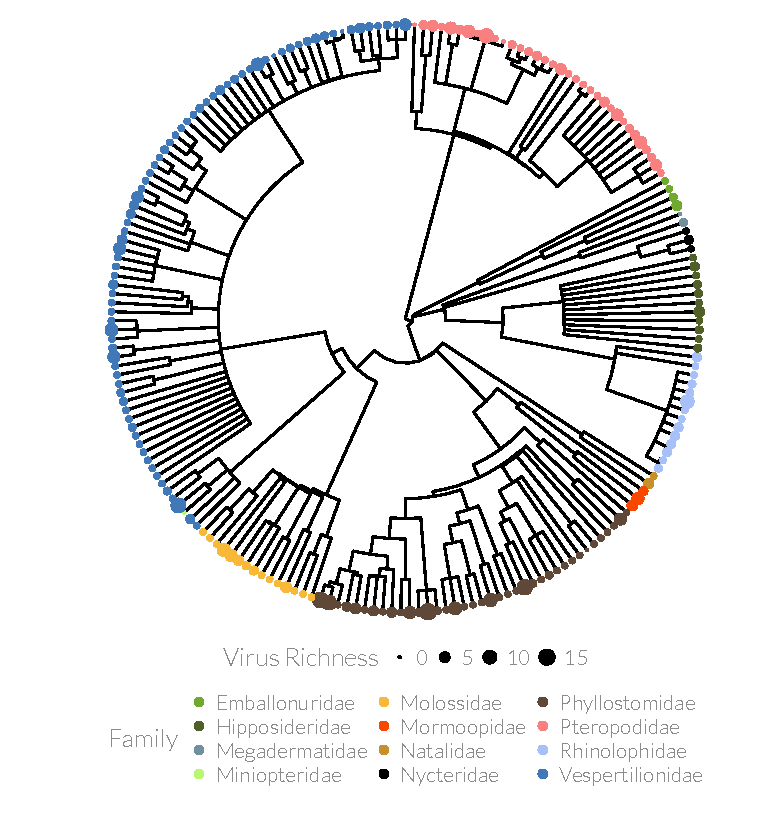
\includegraphics[width=\textwidth]{figure/treePlot-1} 

}

\caption[Pruned phylogeny with dot size showing number of pathogens and colour showing family]{Pruned phylogeny with dot size showing number of pathogens and colour showing family.}\label{fig:treePlot}
\end{figure}


\end{knitrout}












I used two measures of population structure. 
$F_{ST}$ and the number of subspecies.
The number of subspecies was counted using the Wilson and Reeder taxonomy \cite{wilson2005mammal}.
$F_{ST}$ and other measures were collated from the literature.
Studies are from a wide range of spatial scales, from local ($\sim\SI{10}{\kilo\metre}$) to continental.
As $F_{ST}$ inevitably increases with spatial scale I controlled for this by only using data from studies where a large proportion of the species range was studied.
I used the ratio of the furthest distance between $F_{ST}$ samples to the width of the species range and only used studies if this ratio was greater than 0.3.
To allow comparison between different measures ($F_{ST}, \phi_{ST}$) and data from different molecular regions I converted all data to diploid gene flow.
WILL ADD EXTRA METHODS LATER.
These two measures of population structure were analysed separately as the number of subspecies has 196 data points while there is only $F_{ST}$ data for $\sim 30$ bat species.

To control for study bias I collected the number of Pubmed and Google Scholar citations for each bat species including synonyms from ITIS \cite{itis} via the taxize package \cite{chamberlain2013taxize}.
The counts were scraped using the rvest package \cite{rvest}.
I log transformed these variables as they were strongly right skewed.
The log number of citations on Pubmed and Google scholar were highly correlated (pgls: $t$ = 19.32, df = 194, $p$ = 0).
The results here are for analyses using only Google Scholar citations.
See the appendix for analyses run using Pubmed citations.

Measures of body mass are taken from Pantheria \cite{jones2009pantheria} and primary literature \cite{canals2005relative, arita1993rarity, lopez2014echolocation, orr2013does, , lim2001bat, aldridge1987turning, ma2003dietary, owen2003home, henderson2008movements, heaney2012nyctalus, oleksy2015high, zhang2009recent}. 
\emph{Pipistrellus pygmaeus} was assigned the same mass as \emph{P. pipistrellus} as they indistinguishable by mass.
They are log transformed due to the strong right skew.



%Pubmed was scraped on pubmedScrapeDate and Google Scholar was scraped on scholarScrapeDate

To control for phylogenetic nonindependance I used the best-supported phylogeny from \cite{fritz2009geographical} which is the supertree from \cite{bininda2007delayed} with names updated to match the Wilson \& Reeder taxonomy \cite{wilson2005mammal}.
Phylogenetic manipulation was performed using the ape package \cite{ape}.
The importance of the phylogeny on each variable separately was estimated using \cite{phytools}.

I ran two models using the caper package \cite{caper} testing the relationship between pathogen richness and log number of subspecies.
All independant variables were log transformed.
I ran phylogenetically controlled, multivariate linear models.
This model was fitted both with and without an interaction term between number of subspecies and study effort.

Plots were created with a combination of \cite{ggplot2, palettetown, dotwhisker, ggtree}





%\clearpage







\begin{knitrout}\footnotesize
\definecolor{shadecolor}{rgb}{0.969, 0.969, 0.969}\color{fgcolor}\begin{figure}[t]

{\centering 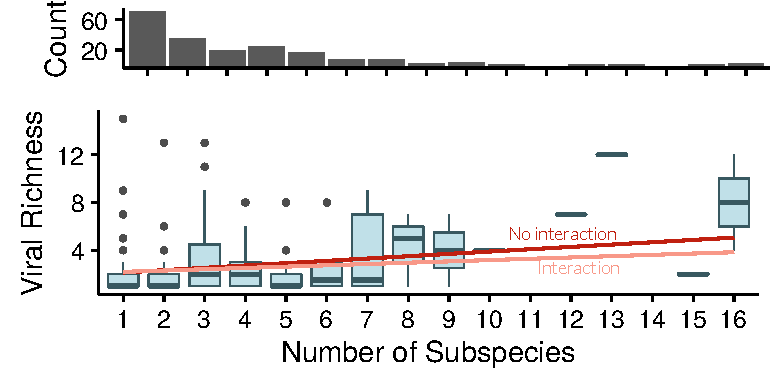
\includegraphics[width=0.8\textwidth]{figure/boxplot-1} 

}

\caption[Number of virus species against number of subspecies]{Number of virus species against number of subspecies. 
Data within a number of subspecies are plotted as boxplots with the dark bar showing the median, the box showing the interquartile range, vertical lines showing the range and outliers shown as seperate points.
Regression lines are from multivariate phylogenetic models with other independant variables set at their median value.
The models shown are thos with (pink) and without (red) an interaction between study effort and number of subspecies.
}\label{fig:boxplot}
\end{figure}


\end{knitrout}



%%being.rcode modelSelectBoots, eval = subBoots

fitModelsBootStrap <- mclapply(1:nBoots, function(b) modelSelect(allFormulae, nSpecies, pruneTree, b, allModelMat, varList), mc.cores = nCores)

allResults <- do.call(rbind, fitModelsBootStrap)

write.csv(allResults, file = 'data/Chapter3/modelSelectSubspecies.csv')


%%end.rcode

\begin{knitrout}\footnotesize
\definecolor{shadecolor}{rgb}{0.969, 0.969, 0.969}\color{fgcolor}

{\centering 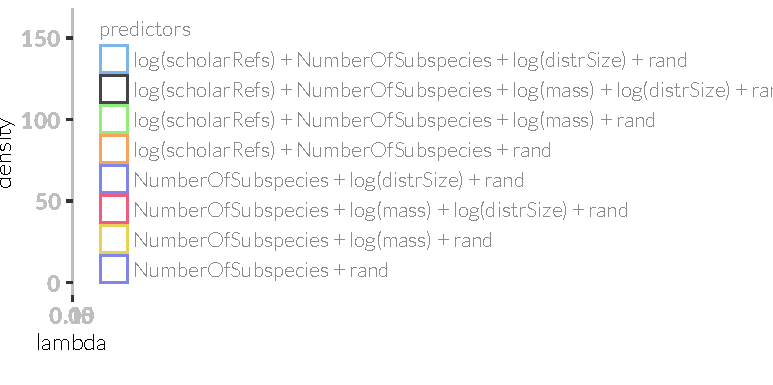
\includegraphics[width=0.8\textwidth]{figure/analyseModelSelect-1} 

}




{\centering 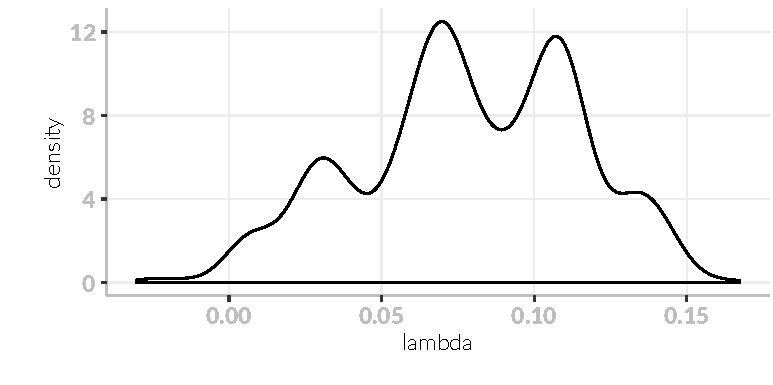
\includegraphics[width=0.8\textwidth]{figure/analyseModelSelect-2} 

}



\end{knitrout}












\clearpage


















\clearpage

%%%%%%%%%%%%%%%%%%%%%%%%%%%%%%%%%%%%%%%%%%%%%%%%%%%%%%%%%%%%%%%%%%%%%%%%%%%%%%%%%%%%%%%%%%%%%%%%%%%%%%%%%%%%%%%%%%%%%%%%%%%%%%%%%%%%%%%%%%%%%%%%%%%%%%%%%%%
%%%% FST ANALYSIS                                                                                                                                  %%%%%%%%
%%%%%%%%%%%%%%%%%%%%%%%%%%%%%%%%%%%%%%%%%%%%%%%%%%%%%%%%%%%%%%%%%%%%%%%%%%%%%%%%%%%%%%%%%%%%%%%%%%%%%%%%%%%%%%%%%%%%%%%%%%%%%%%%%%%%%%%%%%%%%%%%%%%%%%%%%%%









%%%%%%%%%%%%%%%%%%%%%%%%%%%%%%%%%%%%%%%%%%%%%%%%%%%%%%%%%%%%%%%%%%%%%%%%%%%%%%%%%%%%%%%%%%%%%%%%%%%%%%%%%%%%%%%%%%%%%%%%%%%%%%%%%%%%%%%%%%%%%%%%%%%%%%%%%%%

\clearpage
\section{Results}

%%%%%%%%%%%%%%%%%%%%%%%%%%%%%%%%%%%%%%%%%%%%%%%%%%%%%%%%%%%%%%%%%%%%%%%%%%%%%%%%%%%%%%%%%%%%%%%%%%%%%%%%%%%%%%%%%%%%%%%%%%%%%%%%%%%%%%%%%%%%%%%%%%%%%%%%%%%

\subsection{Number of Subspecies}
\tmpsection{More descriptive}

After data cleaning there was data for 196 bat species in 11 families.
The number of described virus species for a bat host ranged up to 15 viruses in \emph{Carollia perspicillata}.
Figure~\ref{fig:treePlot} shows the phylogeny used and the number of viruses for each species.
The mean number of viruses across families is fairly constant with a lower range of 1.67 for Nycteridae.
The highest mean is Mormoopidae with 5 virus species per bat species, but this is based on a sample size of 3.
The Phyllostomidae have the second highest mean (n = 37) of 3.49.

The small change in mean pathogen richness across families and the lack of clear pattern in Figure~\ref{fig:treePlot} implies that viral richness is not strongly phylogenetic. 
This is corroborated by the small estimated size of $\lambda$ ($\lambda$ = , $p$ = ).
This fact implies that other factors must control pathogen richness.
It also implies that pathogens are not directly inherited down the phylogeny, although this is to be expected by the fast evolution of viruses.

Of the explanatory variables, the number of subspecies has no phylogenetic autocorrelation ($\lambda$ = , $p$ = ), study effort has weak but significant autocorrelation ($\lambda$ = , $p$ = ) and mass is strongly phylogenetic ($\lambda$ = , $p$ = ).

\tmpsection{Model results}
See Figure \ref{fig:plotSubspeciesCoefs} for a display of estimated coefficients for the two models using number of viruses as the response variable. 
The main model with mass, study effort and number of subspecies as predictors found study effort to be highly significant ($\beta = $ NA, $p = $ \ensuremath{1.05\times 10^{-8}}). 
The number of subspecies was marginally significant ($\beta = $ NA, $p = $ 0.02). 
The effect of nonindependance due to phylogeny was very small ($\lambda = $ 0.09, $p = $ 0.02).

The interaction term between study effort and number of subspecies, when included, was significant ($\beta = $ 0.14, $p = $ \ensuremath{2.99\times 10^{-3}}).



\subsection{$F_{ST}$}



\begin{knitrout}\footnotesize
\definecolor{shadecolor}{rgb}{0.969, 0.969, 0.969}\color{fgcolor}\begin{figure}[t]

{\centering 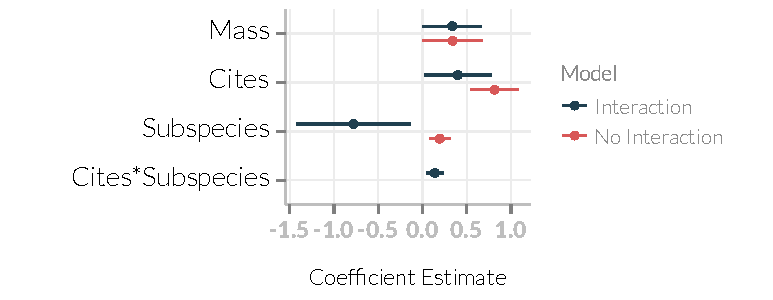
\includegraphics[width=0.8\textwidth]{figure/plotSubspeciesCoefs-1} 

}

\caption[
Plot of coefficient estimates and 95\% confidence intervals for phylogenetic model with and without interactions between study effort and number of subspecies]{
Plot of coefficient estimates and 95\% confidence intervals for phylogenetic model with and without interactions between study effort and number of subspecies. 
Without interactions, number of subspecies is significant.
}\label{fig:plotSubspeciesCoefs}
\end{figure}


\end{knitrout}







\begin{table}[t]
  \rowcolors{2}{gray!25}{white}
  \begin{tabular}{lrr}
  \hline
  Covariate & Estimate (95\% CI) & $p$ value\\
  \hline
  Number of subspecies & 0.19 (0.07 -- 0.32) & \ensuremath{1.94\times 10^{-3}}\\
  Mass & 0.34 (\ensuremath{-1.59\times 10^{-3}} -- 0.68) & 0.05\\
  Study effort & 0.81 (0.54 -- 1.09) & \ensuremath{2.45\times 10^{-8}}\\
  Intercept & \ensuremath{-4.14} (\ensuremath{-6.1} -- \ensuremath{-2.18}) & \ensuremath{5.05\times 10^{-5}}\\
  \end{tabular}
\caption{Table of parameter estimates.}
\label{t:params}
\end{table}








%%%%%%%%%%%%%%%%%%%%%%%%%%%%%%%%%%%%%%%%%%%%%%%%%%%%%%%%%%%%%%%%%%%%%%%%%%%%%%%%%%%%%%%%%%%%%%%%%%%%%%%%%%%%%%%%%%%%%%%%%%%%%%%%%%%%%%%%%%%%%%%%%%%%%%%%%%%

\clearpage
\section{Discussion}  

%%%%%%%%%%%%%%%%%%%%%%%%%%%%%%%%%%%%%%%%%%%%%%%%%%%%%%%%%%%%%%%%%%%%%%%%%%%%%%%%%%%%%%%%%%%%%%%%%%%%%%%%%%%%%%%%%%%%%%%%%%%%%%%%%%%%%%%%%%%%%%%%%%%%%%%%%%%









